\documentclass[problem]{mcs}

\begin{pcomments}
  \pcomment{FP_college_probability}
  \pcomment{F03.q2.prob5}
  \pcomment{adapted by Steven F09}
  \pcomment{problem reworded, solution to tree diagram added, 4/29/14}
\end{pcomments}

\pkeywords{
  probability
  conditional_probability
  tree_diagram
  independence
}

%%%%%%%%%%%%%%%%%%%%%%%%%%%%%%%%%%%%%%%%%%%%%%%%%%%%%%%%%%%%%%%%%%%%%
% Problem starts here
%%%%%%%%%%%%%%%%%%%%%%%%%%%%%%%%%%%%%%%%%%%%%%%%%%%%%%%%%%%%%%%%%%%%%

\begin{problem}
Sally Smart just graduated from high school.  She was accepted to three reputable colleges.

\begin{itemize}

\item With probability $4/12$, she attends Yale.

\item With probability $5/12$, she attends MIT.

\item With probability $3/12$, she attends Little Hoop Community College.

\end{itemize}

Sally is either happy or unhappy in college.

\begin{itemize}

\item If she attends Yale, she is happy with probability $4/12$.

\item If she attends MIT, she is happy with probability $7/12$.

\item If she attends Little Hoop, she is happy with probability
$11/12$.

\end{itemize}

\bparts

\ppart A tree diagram to help Sally project her chance at happiness is
shown below.  On the diagram, fill in the edge probabilities, and at
each leaf write the probability of the corresponding outcome.\iffalse
and happiness event label (``H" for happy, ``U" for unhappy).\fi

\instatements{
\begin{figure}[h]
\graphic[height=2in]{q2-sally}
\end{figure}
}
%\examspace

\begin{solution}
See Figure~\ref{fig:sally-soln}.
\begin{figure}[h]%t!]
%\centering
%\graphic[height=2in]{q2-sally-soln.jpg}
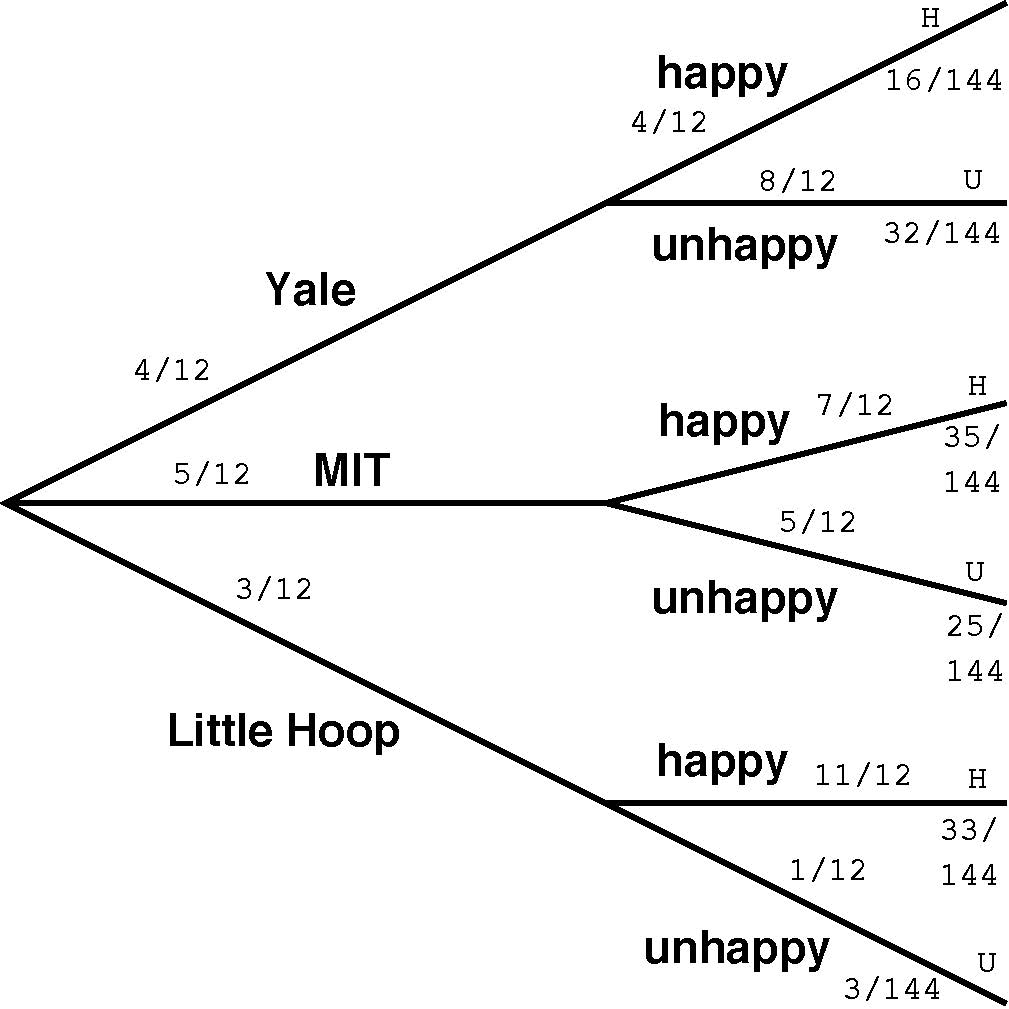
\includegraphics[height=2in]{q2-sally-soln.jpg}
%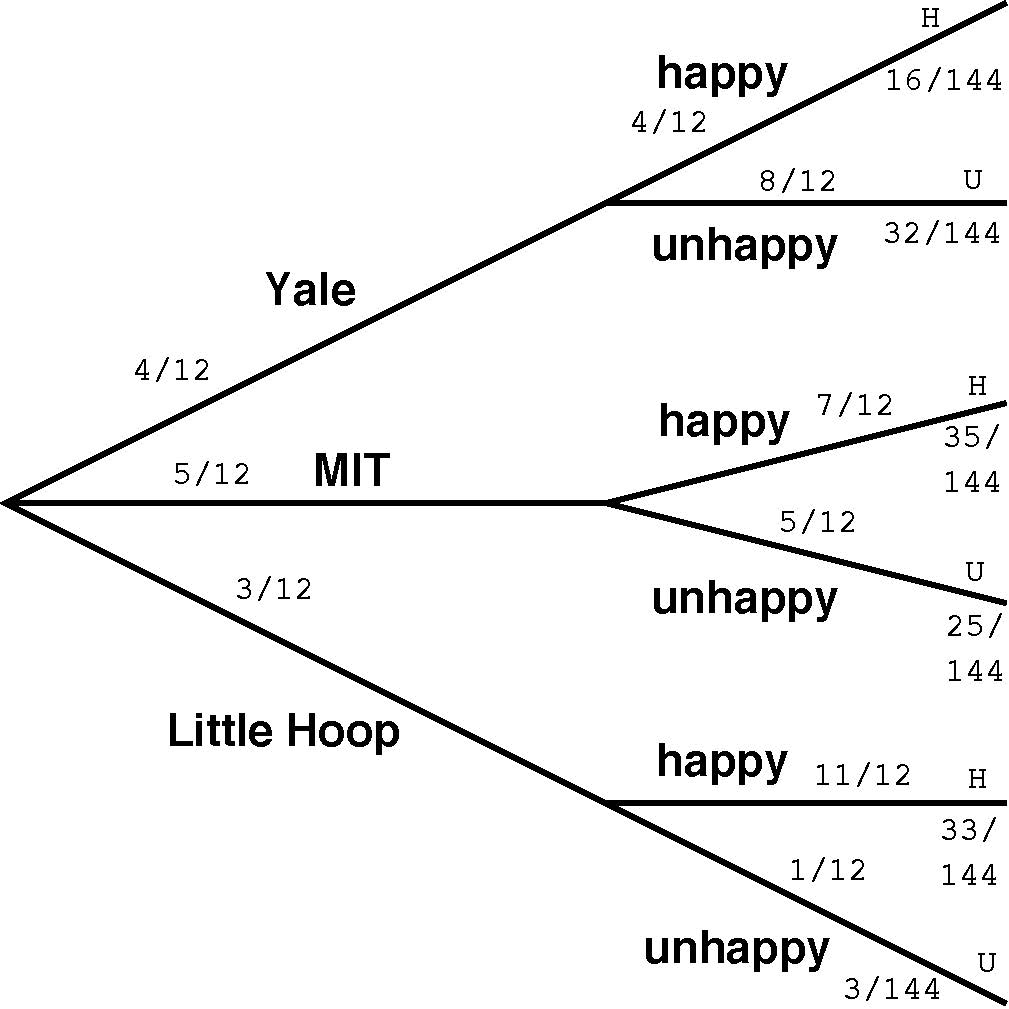
\includegraphics[width=1.2in, left]{q2-sally-soln.jpg}
\caption{Probability tree for College happiness}
\label{fig:sally-soln}
\end{figure}

\end{solution}

\ppart What is the probability that Sally is happy in college?
\examspace[2in]

\begin{solution}
The probability that Sally is happy is equal to
the sum of the probabilities of the outcomes marked with an ``H": $16/144
+ 35/144 + 33/144 = 84/144 = 7/12$.
\end{solution}

\ppart What is the probability that Sally attends Yale, given
that she is happy in college?
\examspace[2in]

\begin{solution}
\begin{align*}
\pr{\text{attends Yale} \mid \text{happy}}
	& =  \frac{\pr{\text{attends Yale} \cap \text{happy}}}
		{\pr{\text{happy}}} \\
	& =  \frac{(4/12) \cdot (4/12)}{(7/12)} \\
	& =  4 / 21
\end{align*}
\end{solution}

\ppart Show that the event that Sally attends Yale \textbf{is not}
independent of the event that she is happy.
\examspace[2in]

\begin{solution}
These two events are independent only if
\[
\pr{\text{attends Yale} \mid \text{happy}} = \pr{\text{attends Yale}}
\]
or $\pr{\text{happy}} = 0$.  However, the left side is $4/21$, the
right side is $4/12$, and the probability that Sally is happy is nonzero.
\end{solution}

\ppart Show that the event that Sally attends MIT \textbf{is}
independent of the event that she is happy.
\examspace[2in]

\begin{solution}
These two events are independent if

\begin{equation*}
\pr{\text{attends MIT}} \cdot \pr{\text{happy}}
	 =  \pr{\text{attends MIT} \cap \text{happy}}
\end{equation*}

The left side is equal to $(5/12) \cdot (7/12) = 35/144$.  According
to the tree diagram, the right side is equal to $35/144$ as well.
\end{solution}

\eparts

\end{problem}

%%%%%%%%%%%%%%%%%%%%%%%%%%%%%%%%%%%%%%%%%%%%%%%%%%%%%%%%%%%%%%%%%%%%%
% Problem ends here
%%%%%%%%%%%%%%%%%%%%%%%%%%%%%%%%%%%%%%%%%%%%%%%%%%%%%%%%%%%%%%%%%%%%%
